\documentclass[12pt, twoside]{article}
\usepackage[letterpaper, margin=1in, headsep=0.2in]{geometry}
\setlength{\headheight}{0.6in}
%\usepackage[english]{babel}
\usepackage[utf8]{inputenc}
\usepackage{microtype}
\usepackage{amsmath}
\usepackage{amssymb}
%\usepackage{amsfonts}
\usepackage{siunitx} %units in math. eg 20\milli\meter
\usepackage{yhmath} % for arcs, overparenth command
\usepackage{tikz} %graphics
\usetikzlibrary{quotes, angles}
\usepackage{graphicx} %consider setting \graphicspath{{images/}}
\usepackage{parskip} %no paragraph indent
\usepackage{enumitem}
\usepackage{multicol}
\usepackage{venndiagram}

\usepackage{fancyhdr}
\pagestyle{fancy}
\fancyhf{}
\renewcommand{\headrulewidth}{0pt} % disable the underline of the header
\raggedbottom
\hfuzz=2mm %suppresses overfull box warnings

\usepackage{hyperref}

\fancyhead[LE]{\thepage}
\fancyhead[RO]{\thepage \\ Name: \hspace{4cm} \,\\}
\fancyhead[LO]{BECA / Dr. Huson / Geometry\\*  Unit 1: Segments, length, and area\\* 30 Sept 2022}

\begin{document}

\subsubsection*{1.12 Test: Length and area}
\emph{Show units if given. Show calculation as an equation, starting with a capitalized variable.}
\begin{enumerate}
\subsubsection*{Line segments, length, number lines}

\item Points $A=-13$ and $B=16$ are shown below. Find the length of segment $\overline{AB}$. \par \smallskip
  \begin{tikzpicture}[scale=0.3]
    \draw[<->] (-22,0)--(22,0);
    \foreach \x in {-20, -15,...,20}
      \draw[shift={(\x,0)}] (0pt,-16pt)--(0pt,16pt)node[below=5pt]{$\x$};
    \draw[fill] (-13,0) circle [radius=0.2] node[above]{$A(-13)$};
    \draw[fill] (16,0) circle [radius=0.2] node[above]{$B(16)$};
    \draw[thick] (-13,0)--(16,0);
  \end{tikzpicture} \vspace{2cm}

\item Isosceles $\triangle DOG$ has congruent sides $\overline{DO} \cong \overline{DG}$. Mark the congruencies with tick marks on the diagram.
  \begin{center}
  \begin{tikzpicture}[scale=0.8]
    \draw[thick] (0,0)node[below left]{$D$}--
      (4,0) node[below]{$O$}--
      (58:4) node[above]{$G$}--cycle;
  \end{tikzpicture}
  \end{center} \bigskip

\item Mark and label irrational number $\sqrt{2} = 1.41421356...$ on the number line below.\par  \vspace{1cm}
\begin{tikzpicture}[scale=4]
  \draw[->] (0,0)--(3.1,0);
  \foreach \x in {0, 0.1,...,3.0}
    \draw[shift={(\x,0)}] (0pt,-1pt)--(0pt,1pt);
  \foreach \x in {0, 0.5,...,3.0}
    \draw[shift={(\x,0)}] (0pt,-3pt)--(0pt,3pt)node[below=25pt]{$\x$};
\end{tikzpicture}

\subsubsection*{Perimeter and area}
\item Measure and mark the lengths of the sides of the rectangle in centimeters. Find its area. \par \medskip
  \begin{tikzpicture}
    \draw [thick] (0,0) rectangle (7,3);
  \end{tikzpicture}

\newpage
\item Find the area of the triangle $ABC$. The $\triangle$'s height is $h=11.5$ and its base measures $AB=6.6$.  \par
\begin{tikzpicture}[scale=1]
  \draw[thick]
    (3,0)node[below]{$A$}--
    (6,0)node[below]{$B$}--
    (7,5)node[above]{$C$} --cycle;
  \draw[dashed] (7,0)--(7,5);
  \draw[dashed, ->] (6,0)--(7.5,0);
  \draw (7,0)++(-0.3,0)--++(0,0.3)--+(0.3,0);
  \node at (7,2.2)[right]{$h=11.5$};
  \node at (4.5,0)[below]{$6.6$};
\end{tikzpicture}
  
\item Find the area of the compound rectangular shape. Show the calculation as the sum of two rectangles.
  \begin{flushleft}
  \begin{tikzpicture}[step=0.5]
    \draw[help lines] (0,0) grid (2.5,4.5) (2.5,3) grid (5.5,4.5);
    \draw[thick] (0,0)--(2.5,0)--(2.5,3)--(5.5,3)--(5.5,4.5)--(0,4.5)--cycle;
    \node at (1.25,-0.5){5};
    \node at (4,2.5){6};
    \node at (5.8, 3.8){3};
    \node at (-0.25, 2.3){9};
  \end{tikzpicture}
  \end{flushleft} \vspace{1cm}

\item Given the circle $O$ with radius $r=5$. Leave exact answers, in terms of $\pi$.
  \begin{multicols}{2}
    \begin{enumerate}
      \item Find the circumference of circle $A$. \vspace{1cm}
      \item Find the area of the circle.\vspace{2cm}
    \end{enumerate}
    \begin{flushright}
    \begin{tikzpicture}[scale=.9]
      \draw (0,0) circle [radius=3];
      \draw[fill] (0,0) circle [radius=0.05] node[below left]{$O$};
      \draw[thick, -{>[scale=1.5]}] (0,0)--(30:3);
      \node at (2,0.5){$r=5$};
    \end{tikzpicture}
  \end{flushright}
  \end{multicols}

\newpage
\item A triangle with 12 centimeter base and $9 \frac{1}{3}$ cm height lies on top of a rectangle with the same base $AB=12$ cm and a width of $2 \frac{1}{2}$ cm. Find the area of the combined figure. \par \medskip
  \begin{tikzpicture}[scale=1.25]
    \draw (2,0)--(7,0);
    \draw[thick] 
      (2,0)node[left]{$E$}--
      (2,-1)node[left]{$A$}--
      (7,-1)node[right]{$B$}--
      (7,0)node[right]{$C$}--
      (3,3)node[above]{$D$}--(2,0);
    \draw[dashed] (3,0)--(3,3);
    \draw (3,0)++(0.3,0)--++(0,0.3)--+(-0.3,0);
    \node at (3,1)[right]{$h=9 \frac{1}{3}$ cm};
    \node at (4.5,-1)[below]{$12$ cm};
    \node at (7,-0.5)[right]{$2 \frac{1}{2}$ cm};
  \end{tikzpicture} \vspace{1.0cm}

\subsubsection*{Precision, percent error}
\item Round each value to the \emph{nearest thousandth}.
  \begin{multicols}{2}
    \begin{enumerate}
      \item $2 \pi$
      \item $\sqrt{3}$
    \end{enumerate}
  \end{multicols} \bigskip 

\item Find the height in meters of a person 61 inches tall. Round to the \emph{nearest hundredth of a meter} (i.e. nearest centimeter).
\vspace{3cm}

\item A palindrome is a word, phrase, or number that reads the same backwards and forwards. (e.g. ``level'', ``racecar''). Find the \% error in this palindromic approximation of pi. \par \bigskip
  $\displaystyle \pi \approx \frac{666}{212}$ \vspace{1.5cm}
  
\newpage
\subsubsection*{Modeling situations and solving with algebra}
\item The parallelogram $GEOM$ has an area $A=72$ and base $GE=9$. Find its height $h$. \par
  \begin{tikzpicture}[scale=.7]
    \draw[thick, ->] (-1.2,0) -- (9,0) node[below]{$x$};
    \draw[thick, ->] (0,-1.2)--(0,6.4) node[left]{$y$};
    \draw[<->, dashed] (1.5,1)--(1.5,5);
    \draw[thick] (2,1)node[below]{$G$}--(7,1)node[below]{$E$}--
    (8,5)node[above]{$O$}--(3,5)node[above]{$M$}--cycle;
    \node at (4.5,1)[below]{$9$};
    \node at (0.5,3)[right]{$h$};
    \node at (5,3.5){$A=72$};
  \end{tikzpicture}

\item The circle $B$ has an area of $A=36 \pi$ square centimeters. Find the radius $r$.
  \begin{multicols}{2}
    \begin{tikzpicture}[scale=0.8]
      \draw (0,0) circle[radius=3];
      \draw[fill] (0,0) circle [radius=0.08];
      \draw[thick, <->] (120:2.9)--(-0.05,0.15)node[below=5pt]{$B$};
      \draw (0.3,1.8) node[below]{$r=\ ?$};
    \end{tikzpicture} \par
   Start with the formula \par \smallskip
  $A = \pi r^2 = 36 \pi$
  \end{multicols}
  
\item Given $\overline{PQR}$, with $PQ=2x+4$, $QR=x+3$, and $PR=22$. Find ${PQ}$. (show check) \par \bigskip
  \begin{tikzpicture}
    \draw[thick] (0,0)--(6,0);
    \draw[fill] (0,0) circle [radius=0.05] node[below]{$P$};
    \draw[fill] (4,0) circle [radius=0.05] node[below]{$Q$};
    \draw[fill] (6,0) circle [radius=0.05] node[below]{$R$};
    \node at (2,0.5){$2x+4$};
    \node at (5,0.5){$x+3$};
    \draw[<->, dashed] (0,-1)--(6,-1);
    \node at (3,-1) [below]{$22$};
  \end{tikzpicture}


\end{enumerate}
\end{document}